\documentclass[12pt, a4paper, onecolumn, oneside, final]{report}
\usepackage{graphicx}
\usepackage{array}

\usepackage{ragged2e}

\begin{document}

\chapter{Pendahuluan}
\justifying
\section{Latar Belakang}
\par  Perkembangan teknologi informasi dan komunikasi di Indonesia semakin pesat, dan kebutuhan akan informasi yang cepat sangat dibutuhkan oleh masyarakat. Begitu juga kebutuhan akan komunikasi yang cepat dan akurat untuk menyediakan data yang valid, khususnya dalam sebuah instansi. Akses yang cepat dan akurat kini dapat diperoleh melalui teknologi yang terkoneksi dengan internet. Teknologi banyak dimanfaatkan sebagai sistem informasi, salah satunya dengan menggunakan teknologi web, di mana informasi dapat diakses tanpa batasan ruang dan waktu, seperti dalam metode pemrograman untuk membangun aplikasi menggunakan komputer.
\par Perumahan merupakan salah satu kebutuhan utama manusia yang harus di penuhi di samping pangan dan sandang, artinya setiap orang sangat memerlukan tempat tinggal atau rumah untuk berteduh dari panas dan hujan.rumah adalah bangunan yang berfungsi sebagai tempat tinggal atau hunian dan sarana pembinaan keluarga sedangkan perumahan adalah kelompok rumah yang berfungsi sebagai lingkungan tempat tinggal atau lingkungan hunian yang dilengkapi dengan sarana dan prasarana dan permukiman adalah bagian dari lingkungan hidup di luar kawasan lindung, baik berupa kawasan perkotaan maupun perdesaan yang berfungsi sebagai tempat tinggal atau hunian dan tempat kegiatan yang mendukung perikehidupan dan penghidupan (UU no. 4 tahun 1992 tentang perumahan dan pemukiman,pasal 1 ayat 2).
\par Perumahan Kamela Permai merupakan sebuah perumahan yang berada di Kabupaten Kuantan Singingi. Berdasarkan observasi langsung oleh peneliti di Perumahan Kamela Permai Bangkinang Bersama Agusman, S.E selaku Kepala Cabang, pemesanan perumahan masih dilakukan secara manual dan harus mendatangi kantor marketing untuk mendapatkan syarat-syarat pemesanan.. Hal ini menyebabkan calon pelanggan yang jauh dari lokasi perumahan sulit untuk mengetahui dan melakukan pemesanan. Oleh karena itu, diperlukan sistem informasi pemesanan perumahan agar pemesananan dapat menjangkau calon pelanggan lebih luas dan lebih mudah. Selain itu sistem informasi ini juga menyimpanan dokumen yang dipelukan untuk pemesanan hingga dapat dicari dengan mudah oleh marketing.
\par Dari uraian tersebut, penulis tertarik untuk membangun sebuah sistem informasi pemesanan perumahan sehingga permasalahan yang dihadapi dapat diselesaikan. Oleh karena itu, penulis mengangkatnya menjadi materi Laporan Kerja Praktek dengan judul “Rancang Bangun Sistem Informasi Pemesanan Perumahan” yang diharapkan dapat mempermudah proses pemesanan perumahan di Perumahan Kamea Permai.

        \begin{figure}
        \centering
        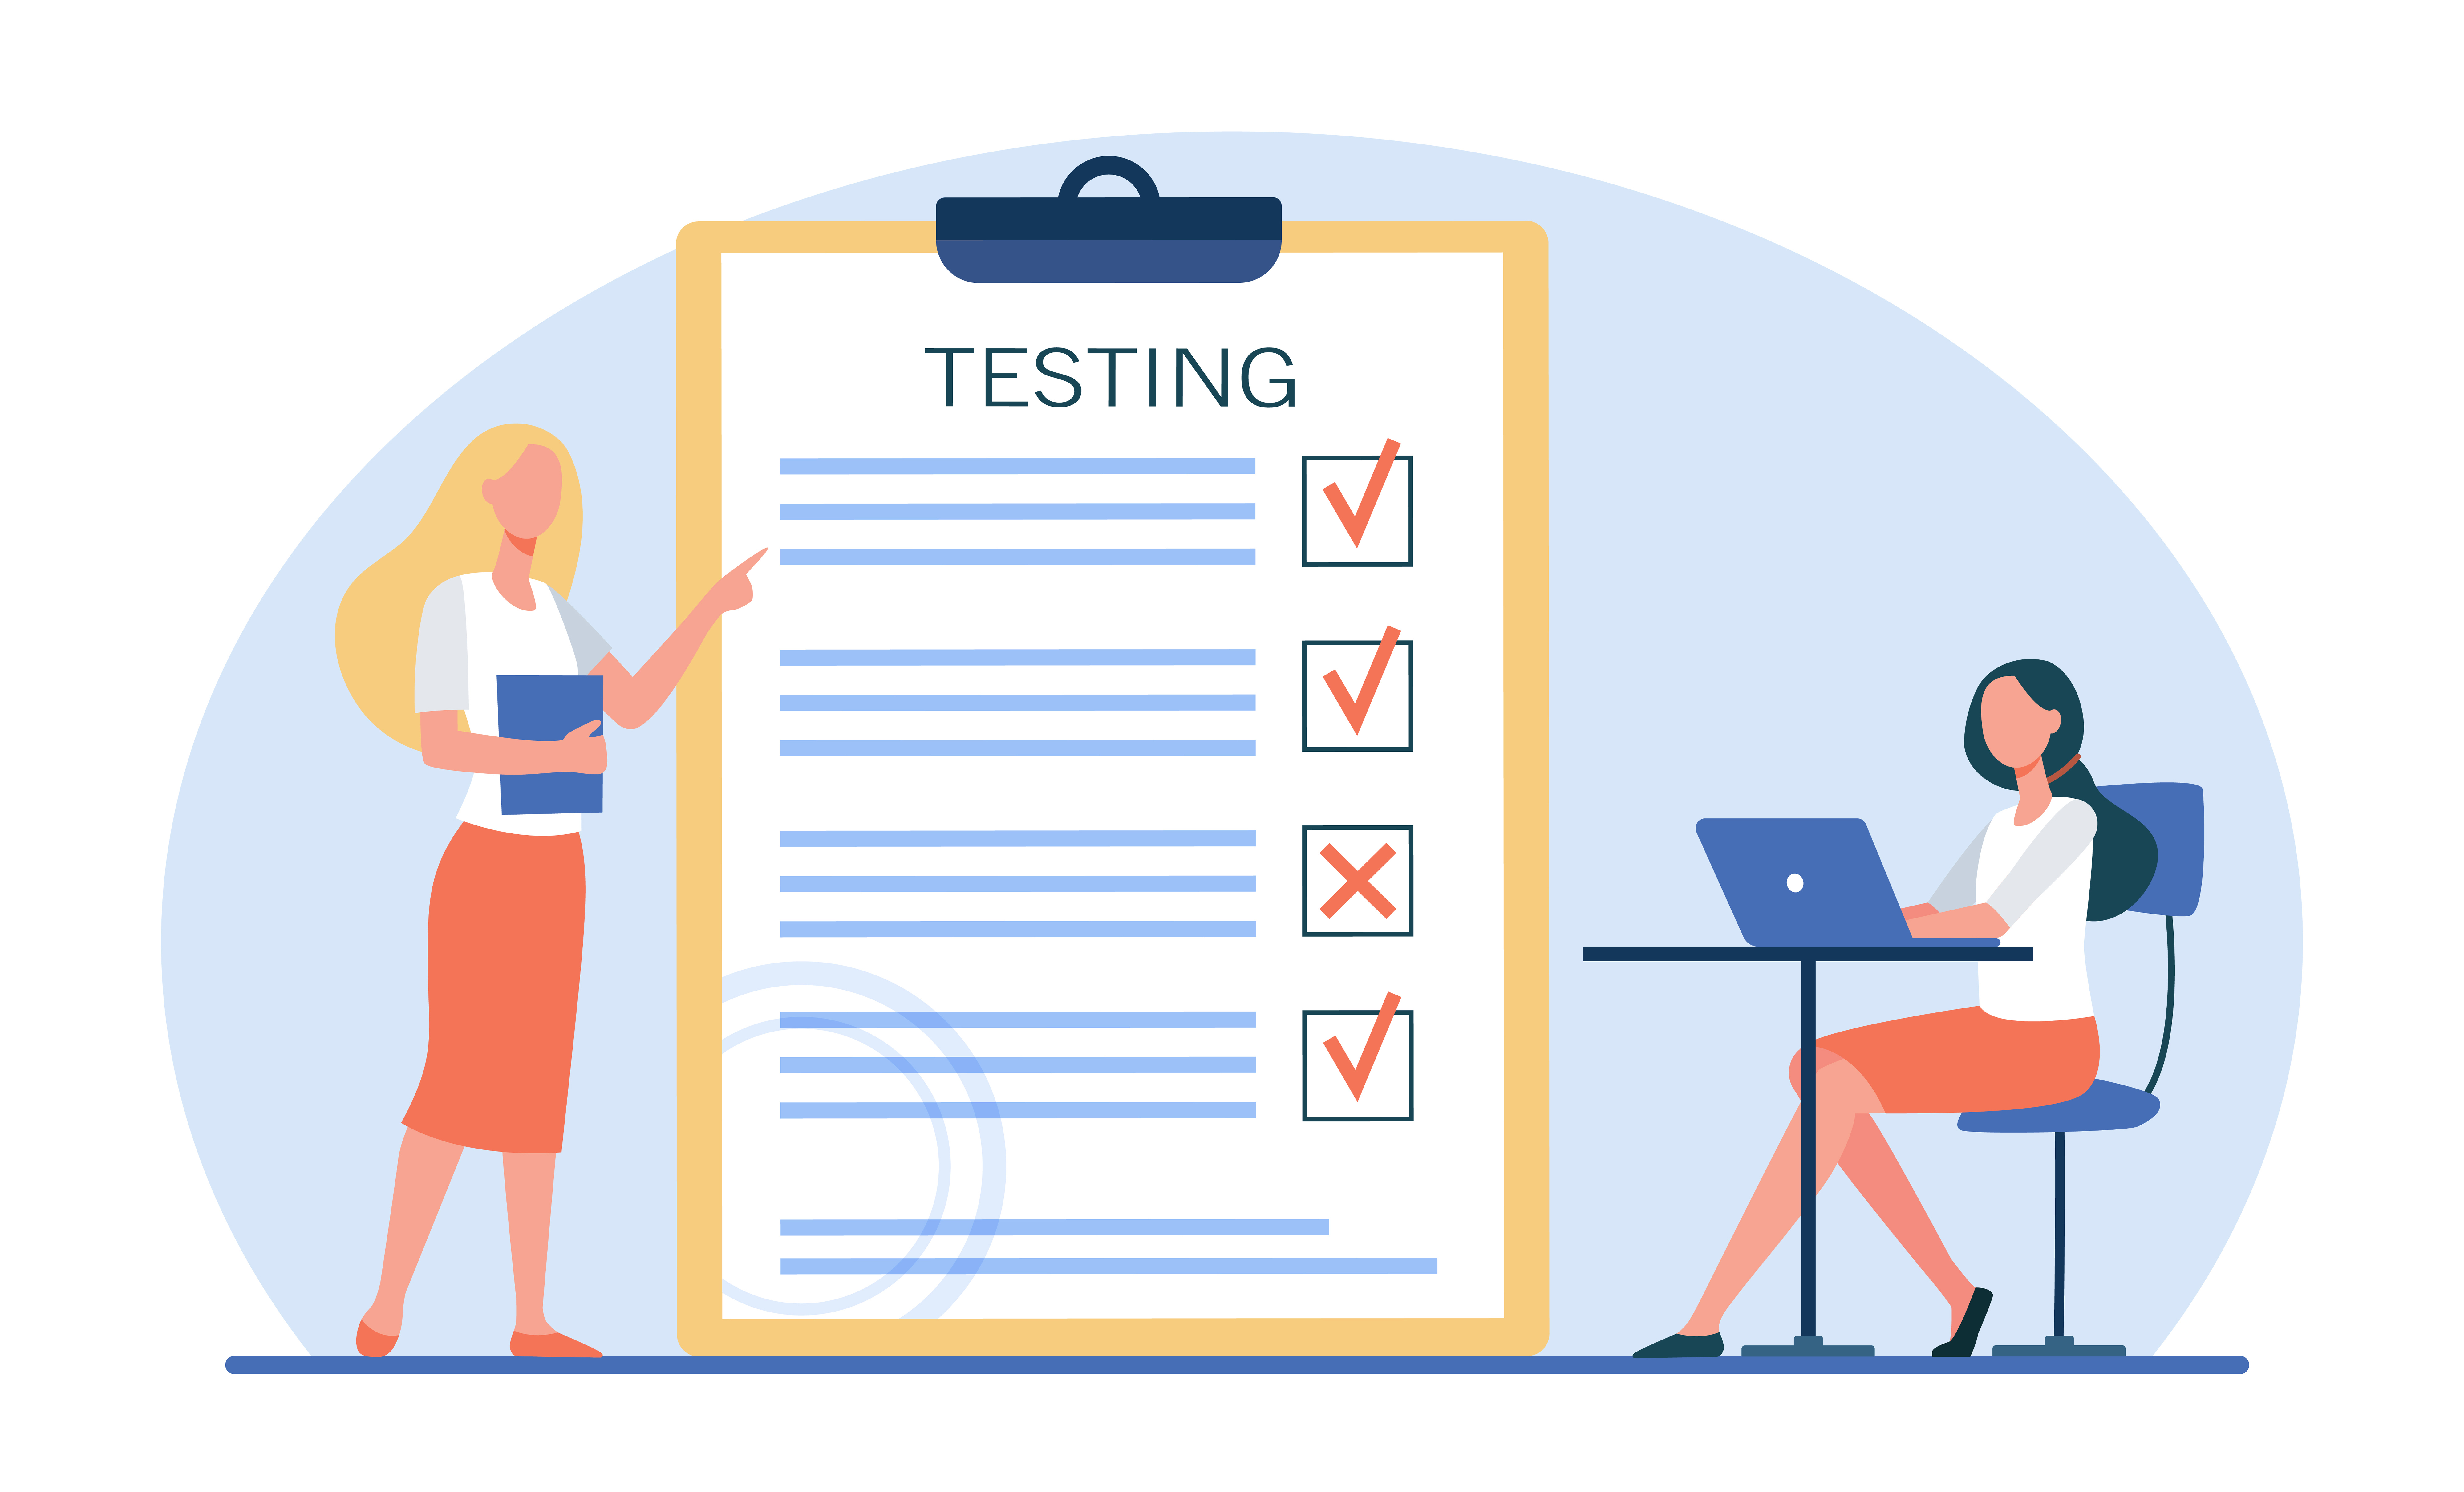
\includegraphics[width=10cm]{test.jpg}
        \caption{contoh gambar}
        \end{figure}
        \section{Rumusan Masalah}
\par  Berdasarkan uraian latar belakang di atas, dapat dirumuskan permasalahannya yaitu “Bagaimana merancang dan membangun Bangun Sistem Informasi Pemesanan Perumahan di Perumahan Kamela Permai”?
\section{Batasan Masalah}
\par  Dalam perancangan dan penulisan laporan kerja praktek ini, pembahasan masalah memiliki beberapa batasan permasalahan, antara lain:
\begin{enumerate}
\item \par Sistem yang dibangun merupakan sistem terkomputerisasi yang berfokus pada Pemesanan Perumahan.

\item \par Sistem yang dibangun adalah berbasis web dengan menggunakan bahasa pemrograman \textit{PHP} dengan \textit{Http Library Oktaax} dan database \textit{MYSQL}.

\item \par Metode analisis dan perancangan yang digunakan adalah \textit{Unified Modeling Language (UML)} dengan hanya menggunakan tiga jenis diagram, yaitu: \textit{Use Case Diagram, Activity Diagram}, dan \textit{Class Diagram}.

\item \par Perancangan sisem ini dibuat dengan menggunakan Metode \textit{Extreme Programming} hingga tahap pengujian.

\end{enumerate}
\section{Tujuan}
\par  Adapun tujuan pelaksanaan kerja praktek adalah:
\begin{enumerate}
\item \par Untuk membangun sebuah Sistem Informasi Pemesanan Rumah di Perumahan Kamela Permai.

\item \par Untuk mengetahui keberhasilan menggunakan metode Extreme Programming dalam membangun sebuah Sistem Informasi Pemesanan Perumahan.

\end{enumerate}
\section{Manfaat}
\par  Adapun manfaat penulis melakukan kerja praktek ini adalah:
\begin{enumerate}
\item \par Dapat mempermudah calon pembeli dalam memesan rumah di perumahan Kamela Permai.

\item \par Dapat melihat informasi pemesanan rumah secara up to date.

\end{enumerate}
\section{Sistematika Penulisan}
\par  Sistematika penulisan laporan kerja praktek ini dibagi menjadi 5 (lima) bab. Berikut penjelasan tentang masing-masing bab: BAB 1. Pendahuluan Dalam bab ini penulis memaparkan tentang latar belakang, rumusan masalah, batasan masalah, tujuan, manfaat, tempat dan waktu pelaksanaan serta sistematika penulisan laporan kerja praktek. \textbf{BAB 2. }\textbf{Landasan Teori} Bab ini menjelaskan beberapa teori yang berkaitan dengan penelitian, teori yang bersifat umum dan berkaitan dengan topik penelitian hingga teori yang bersifat khusus dalam kaitan proses pembuatan sistem informasi. \textbf{BAB 3. }\textbf{Tugas Kerja Praktek} Bab ini menjelaskan mengenai gambaran dari pelaksanaan kerja praktek yang akan dilakukan kurang lebih selama satu setengah bulan. \textbf{BAB 4. }\textbf{Analisa dan Hasil} Pada bab ini menguraikan beberapa analisis yang dibutuhkan dalam membangun sistem informasi. \textbf{BAB 5. }\textbf{PENUTUP} Bab ini berisikan kesimpulan mengenai hasil dari perancangan aplikasi yang telah dibuat, dan saran dari pembaca apabila ingin mengembangkan aplikasi ini lebih lanjut.

\end{document}

